\documentclass[a4paper,12pt]{article} % тип документа
\usepackage{wrapfig}
\usepackage{tikz}
\usepackage[T2A]{fontenc}			% кодировка
\usepackage[utf8]{inputenc}			% кодировка исходного текста
\usepackage[english,russian]{babel}	% локализация и переносы
\usepackage{amsfonts,longtable}

% Математика
\usepackage{amsmath,amsfonts,amssymb,amsthm,mathtools} 


\usepackage{wasysym}

\title{Лабораторная работа 1.2.5 по курсу \\ "Общая физика"  \\ 
\vspace{0.2cm}
\vspace{4.5cm}
 \LARGE{\textbf{Исследование прецессии уравновешенного гироскопа}}\vspace{5.5cm}}
\date{14.12.2018}
\usepackage{tikz}
\author{\vspace{0.2cm}Баринов Леонид}

\begin{document}
\maketitle
\newpage
\section{Аннотация}
В работе будет исследована вынужденная прецессия гироскопа; установлены зависимости скорости вынужденной прецессии от величины момента сил, действующих на ось гироскопа; определена скорость вращения ротора гироскопа и будет проведено сравнение ее со скоростью, рассчитанной по скорости прецессии. Также будет проведена оценка влияния момента силы трения на прецессию гироскопа.
\section{Теоретические сведения}
Уравнения движения твердого тела можно записать в виде:
\begin{equation}
\frac{\overrightarrow{P}}{dt} = \overrightarrow{F}
\end{equation}
\begin{equation}
\frac{d\overrightarrow{L}}{dt} = \overrightarrow{M}
\end{equation}
Здесь (1) выражает закон движения центра масс тела, а (2) — уравнение моментов. Поскольку твердое тело имеет только шесть степеней свободы, этих двух векторных уравнений достаточно для полного описания состояния его движения.

Если сила $\overrightarrow{F}$ не зависит от угловой скорости, а момент $\overrightarrow{M}$ — от скорости поступательного движения, то уравнения (1) и (2) можно рассматривать независимо друг от друга. В баллистике, например при движении снаряда в воздухе, это невозможно. В случае же, когда такое раздельное рассмотрение возможно, уравнение (1) соответствует просто задаче о движении материальной точки, а уравнение (2) — задаче о вращении твердого тела вокруг неподвижной точки. В данной работе рассматривается последняя из этих задач.

Момент импульса твердого тела в его главных осях$ х, у, z$ равен
\begin{equation}
\overrightarrow{L} = \overrightarrow{i}I_x\omega_x+\overrightarrow{j}I_y\omega_y + \overrightarrow{k}I_z\omega_z
\end{equation}
где $I_x, I_y, I_z$ — главные моменты инерции. usx, иу, u>z — компонента: вектора угловой скорости й. Быстро вращающееся тело, для которого, например,
\[I_z\omega_z \gg I_x\omega_x, I_y\omega_y\]
принято называть гироскопом. Гироскоп называется уравновешенным, если его центр масс неподвижен.

В силу (2) приращение момента импульса определяется интегралом
\begin{equation}
\Delta\overrightarrow{L} = \int\overrightarrow{M}dt
\end{equation}
Если момент внешних сил действует в течение короткого промежутка времени, из интеграла (4) следует, что приращение $\Delta\overrightarrow{L}$ момента импульса значительно меньше самого момента импульса:
\[|\Delta\overrightarrow{L}| \ll |\overrightarrow{L}|\]
С этим связана замечательная устойчивость, которую приобретает движение гироскопа после приведения его в быстрое вращение.
\begin{wrapfigure}{r}{0.5\textwidth}
  \begin{center}
    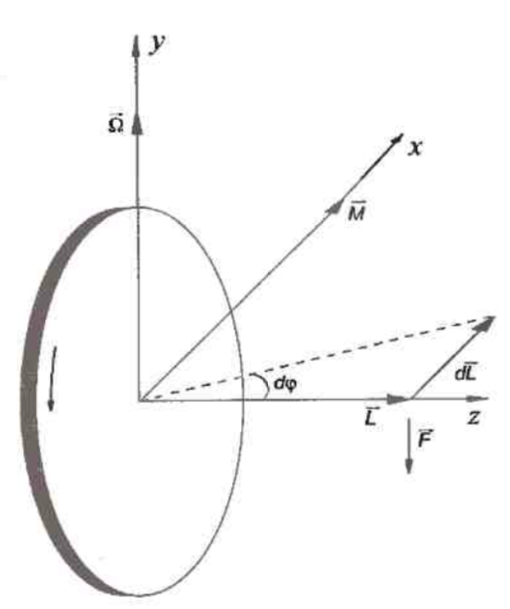
\includegraphics[width=0.48\textwidth]{1}
  \end{center}
  \caption{Маховик}
\end{wrapfigure}

Выясним, какие силы надо приложить к гироскопу, чтобы изменить направление его оси. Рассмотрим для примера маховик, вращающийся вокруг оси $z$, перпендикулярной к плоскости маховика (рис. 1). Будем считать, что
\[\omega_z = \omega_0, \quad \omega_x = 0, \quad \omega_y = 0.\]
Пусгь ось вращения повернулась в плоскости $zx$ по направлению к оси $х$ на бесконечно малый угол $d\varphi$. Такой поворот означает добавочное вращение маховика вокруг оси $y$, так что
\[d\varphi = \Omega dt,\]
где $\Omega$ — угловая скорость такого вращения. Будем предполагать, что
\begin{equation}
L_\Omega \ll L_{\omega_0}
\end{equation}
Это означает, что момент импульса маховика, равный $I_z\omega_0$ до приложения внешних сил, только повернется в плоскости $zx$ по направлению к оси $х$ не изменяя своей величины. Таким образом,
\[|d\overrightarrow{L}| = Ld\varphi = L\Omega dt\]
Но это изменение направлено вдоль оси $x$, поэтому вектор $d\overrightarrow{L}$ можно представить в виде векторного произведения вектора угловой скорости $\overrightarrow{\Omega}$, направленного вдоль оси $y$, на вектор собственного момента импульса маховика, направленного вдоль оси $z$,
\[d\overrightarrow{L} = \overrightarrow{\Omega} \times \overrightarrow{L}dt,\]
т. е.
\[\frac{d\overrightarrow{L}}{dt} = \overrightarrow{\Omega} \times \overrightarrow{L}\]
В силу (2) имеем
\begin{equation}
\overrightarrow{M} = \overrightarrow{\Omega} \times \overrightarrow{L}
\end{equation}
Формула (6) справедлива, если выполнено условие (5). Она позволяет определить момент сил $\overrightarrow{M}$, который необходимо приложить к маховику для того, чтобы вызвать вращение оси маховика с угловой скоростью $\overrightarrow{\Omega}$. Мы видим, таким образом, что для поворота оси вращающегося маховика к оси $x$ необходимо приложить силы, направленные не вдоль оси $x$, а вдоль оси $у$, так чтобы их момент $\overrightarrow{M}$ был направлен вдоль оси $x$.

Под действием момента $\overrightarrow{M}$ внешних сил ось гироскопа медленно вращается вокруг оси $у$ с угловой скоростью $\Omega$. Такое движение называется регулярной прецессией гироскопа. В частности, создающей момент внешней силой может оказаться сила тяжести, если центр масс гироскопа не совпадает с точкой подвеса. Для гироскопа массой $m_\text{г}$, у которого ось собственного вращения наклонена на угол $\alpha$ от вертикали, скорость прецессии, происходящей вокруг вертикальной оси под действием силы тяжести, равна
\begin{equation}
\Omega = \frac{M}{I_z\omega_0\sin\alpha}= \frac{m_\text{г}gl_\text{ц}\sin\alpha}{I_z\omega_0\sin\alpha} = \frac{m_\text{г}gl_\text{ц}}{I_z\omega_0}
\end{equation}
где $l_\text{ц}$ — расстояние от точки подвеса до центра масс гироскопа, т. е. скорость прецессии не зависит от угла $\alpha$.

Для изучения регулярной прецессии уравновешенного гироскопа к его оси подвешивают дополнительные грузы. Это смещает общий центр масс и создает момент сил тяжести, вызывающий прецессию. Скорость прецессии в этом случае равна
\begin{equation}
\Omega = \frac{mgl}{I_z\omega_0}
\end{equation}
где $m$ — масса груза, $l$— расстояние от центра карданова подвеса до точки крепления груза на оси гироскопа (рис. 3).

\section{Экспериментальная установка}

В данной работе исследуется регулярная прецессия уравновешенного гироскопа.

Уравновешенный гироскоп, закрепленный в кольцах карданова подвеса, показан на рис. 2. Наружное кольцо подвеса $\text{А}$ может свободно поворачиваться вокруг вертикальной оси $aa$. Внутреннее кольцо $\text{Б}$ связано с кольцом $\text{А}$ горизонтальной осью $\text{бб}$. В кольце $\text{Б}$ укреплен гироскоп, ось вращения которого $\text{вв}$ перпендикулярна к оси $\text{бб}$. Центр масс гироскопа находится на пересечении всех трех осей и при любом повороте колец сохраняет свое положение в пространстве. Получается, что гироскоп как бы подвешен за центр масс.
\begin{figure}[h]
\centering
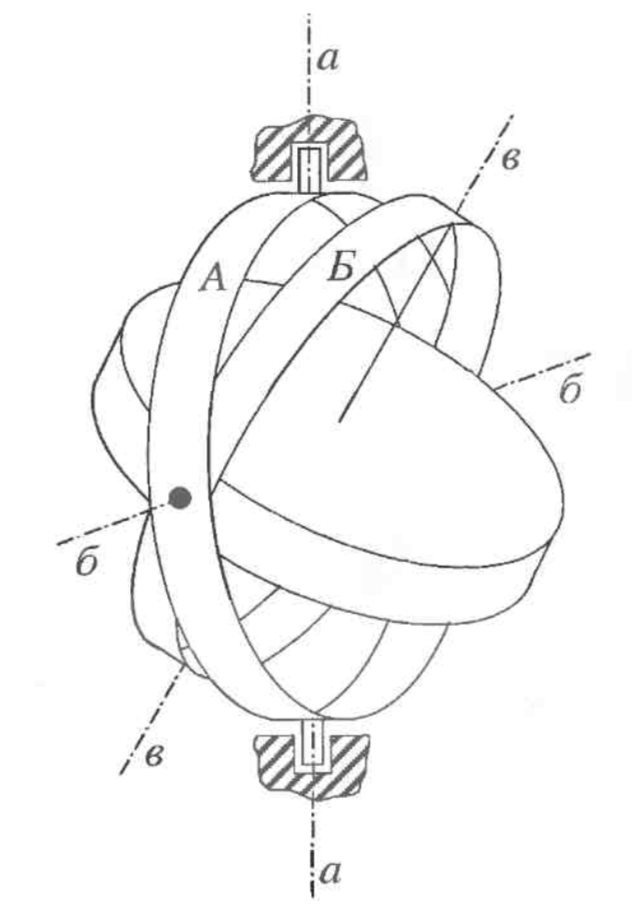
\includegraphics[scale=0.5]{2}
\caption{Гироскоп в кардановом подвесе}
\end{figure}

Экспериментальная установка для исследования прецессии уравновешенного гироскопа показана на рис. 3. Ротором гироскопа является ротор высокооборотного электромотора $M$, питающегося током частотой $400\text{Гц}$. Кожух мотора (статор, имеющий обмотки, питаемые током частотой $400\text{Гц}$) скреплен с кольцом $\text{Б}$ (рис. 2 и 3). Мотор с кольцом $\text{Б}$ может вращаться в кольце $\text{А}$ вокруг горизонтальной оси $\text{бб}$, которое может вращаться вокруг вертикальной оси $\text{аа}$. Ротор электромотора представляет массивный стальной цилиндр с прожилками меди, образующими «беличье колесо». Обозначенный на рис. 3 буквой $\text{С}$ рычаг направлен по оси симметрии ротора. На рычаг подвешивают грузы $\text{Г}$. Подвешивая различные грузы, можно менять силу $F$, момент которой определяется расстоянием $I$ от точки подвеса до горизонтальной оси кольца $\text{А}$ (до центра масс гироскопа), указанным на самой установке.

Выше при выводе формул для прецессии предполагалось, что действующие на гироскоп силы лежат в плоскости $zy$, в которой лежат векторы угловых скоростей собственного вращения и прецессии. В этом случае, как уже говорилось, момент сил меняет лишь направление момента импульса гироскопа, но не его величину. Силы трения не лежат в плоскости осей вращения. Они приводят к изменению момента импульса и по направлению, и по величине. Для ротора гироскопа действие сил трения скомпенсировано действием электромотора. Для осей карданова подвеса компенсации нет. В результате ось гироскопа будет опускаться в направлении действия груза. 

В первой части работы исследуется зависимость скорости прецессии гироскопа от момента силы, приложенной к его оси. Для этого к оси гироскопа (к рычагу $\text{С}$) подвешиваются грузы $\text{Г}$. Скорость прецессии определяется по числу оборотов рычага вокруг вертикальной оси и вымени, которое на это ушло, определяемое секундомером. В процессе измерений рычаг не только поворачивается в результате прецессии гироскопа, но и опускается. Поэтому его в начале опыта следует приподнять на $5-6^\circ$. Опыт надо закончить, когда рычаг опустится на такой же угол.

Измерение скорости прецессии гироскопа позволяет вычислить угловую скорость вращения его ротора. Расчет производится по формуле (8). Момент инерции ротора относительно оси симметрии $I_0$ измеряется по крутильным колебаниям точной копии ротора, подвешиваемой вдоль оси симметрии на жесткой проволоке. Период крутильных колебаний $T_0$ зависит от момента инерции $I_0$ и модуля кручения проволоки $f$:
\begin{equation}
T_0 = 2\pi\sqrt{\frac{I_0}{f}}
\end{equation}

Чтобы исключить модуль кручения проволоки, вместо ротора гироскопа к той же проволоке подвешивают цилиндр правильной формы с известными размерами и массой, для которого легко можно вычислить момент инерции $I_\text{ц}$. Для определения момента инерции ротора гироскопа имеем
\begin{equation}
I_0 = I_\text{ц}\frac{T_0^2}{T_{\text{ц}}^2},
\end{equation}
здесь $T_\text{ц}$ -- период крутильных колебаний цилиндра.
\section{Оборудование и инструментальные погрешности}
Расстояние от центра карданова подвеса до точки крепления груза на оси гироскопа:
\[l = 121\text{мм}\]
Масса цилиндра:
\[m_\text{ц} = 1617,8\text{г}\]
\section{Результаты измерений и обработка данных}
Отклоняем рычаг $\text{С}$ на $5-6^{\circ}$ градусов вверх от горизонтальной плоскости. Подвесим к нему груз $\text{Г}$ и с помощью секундомера найдем угловую скорость регулярной прецессии $\text{П}$ (по числу оборотов и времени прецессии). Измерения продолжаем до тех пор, пока рычаг $\text{С}$ не опустится на $5-6^{\circ}$ градусов ниже горизонтальной плоскости, сделав целое число оборотов относительно вертикальной оси.

Проведем серию измерения для груза с $m = 219\text{г}$. Результаты занесем в Таблицу 1. $n$ - число оборотов, которые успеет совершить гироскоп, когда рычаг опуститься на $5-6^{\circ}$.
\begin{table}[h]
\centering
\begin{tabular}{|c|c|c|c|c|c|c|}
\hline
$\text{№}$ & 1      & 2     & 3      & 4      & 5     & 6      \\ \hline
$n$      & 3,5    & 3,5   & 3,5    & 3,5    & 3,5   & 3,5    \\ \hline
$t, \text{с}$      & 220,25 & 223,4 & 220,46 & 220,03 & 220,8 & 222,69 \\ \hline
\end{tabular}
\caption{Измерение времени прецессии $t$ для груза c $m = 219\text{г}$, за которое гироскоп опуститься на $5-6^{\circ}$, совершив при этом $n$ оборотов}
\end{table}

Находим угловую скорость регулярной прецессии $\Omega$ по формуле 
\[\Omega = \frac{2\pi n}{t}\]
Усредняя данные получим, что 
\[\Omega_\text{ср} = (0,099\pm0,001)\text{рад/с}\]
Относительная погрешность равна:
\[\varepsilon = \frac{0,001}{0,099} = 1\%\]
Будем использовать эту оносительную погрешность при вычислениюю угловой скорости регулярной прецесси гироскопа с другими грузами

Проведем серию экспериментов с грузами разной массы. Также посчитаем угловую скорость регулярной прецессии $\Omega$, момент силы действия груза $\text{Г}$ относительно центра масс $M = mgl$, угловую скорость опускания рычага $\Omega_\text{тр} = \frac{\pi/15}{t}$. Результаты занесем в Таблицу 2.
\begin{table}[h]
\centering
\begin{tabular}{|c|c|c|c|c|c|c|}
\hline
$m, \text{г}$   & $n$   & $t, c$      & $\Omega, \text{рад/с}$  & $\sigma_\Omega,\text{рад/с}$     & $M, H\cdot\text{м}$      & $\Omega_\text{тр}, 10^{-3}\text{рад/с}$   \\ \hline
116 & 3   & 356,35 & 0,0529 & 0,00053 & 0,1404 & 0,59 \\ \hline
142 & 3   & 298,05 & 0,0632 & 0,00063 & 0,1718 & 0,70 \\ \hline
180 & 3   & 230,74 & 0,0817 & 0,00082 & 0,2178 & 0,91 \\ \hline
219 & 3,5 & 220,25 & 0,0994 & 0,00099 & 0,2650 & 0,95 \\ \hline
273 & 4   & 208,19 & 0,1207 & 0,00121 & 0,3303 & 1,01 \\ \hline
341 & 4   & 164,08 & 0,1531 & 0,00153 & 0,4126 & 1,28 \\ \hline
\end{tabular}
\caption{Угловая скорость регулярной прецессии гироскопа $\Omega$ для грузиков различной массы}
\end{table}

По результатам Таблицы 2 построим график зависимости угловой скорости регулярной прецессии гироскопа $\Omega$ от момента силы тяжести $M$, который создает грузик. (Рис. 3)

\begin{figure}[h]
\centering
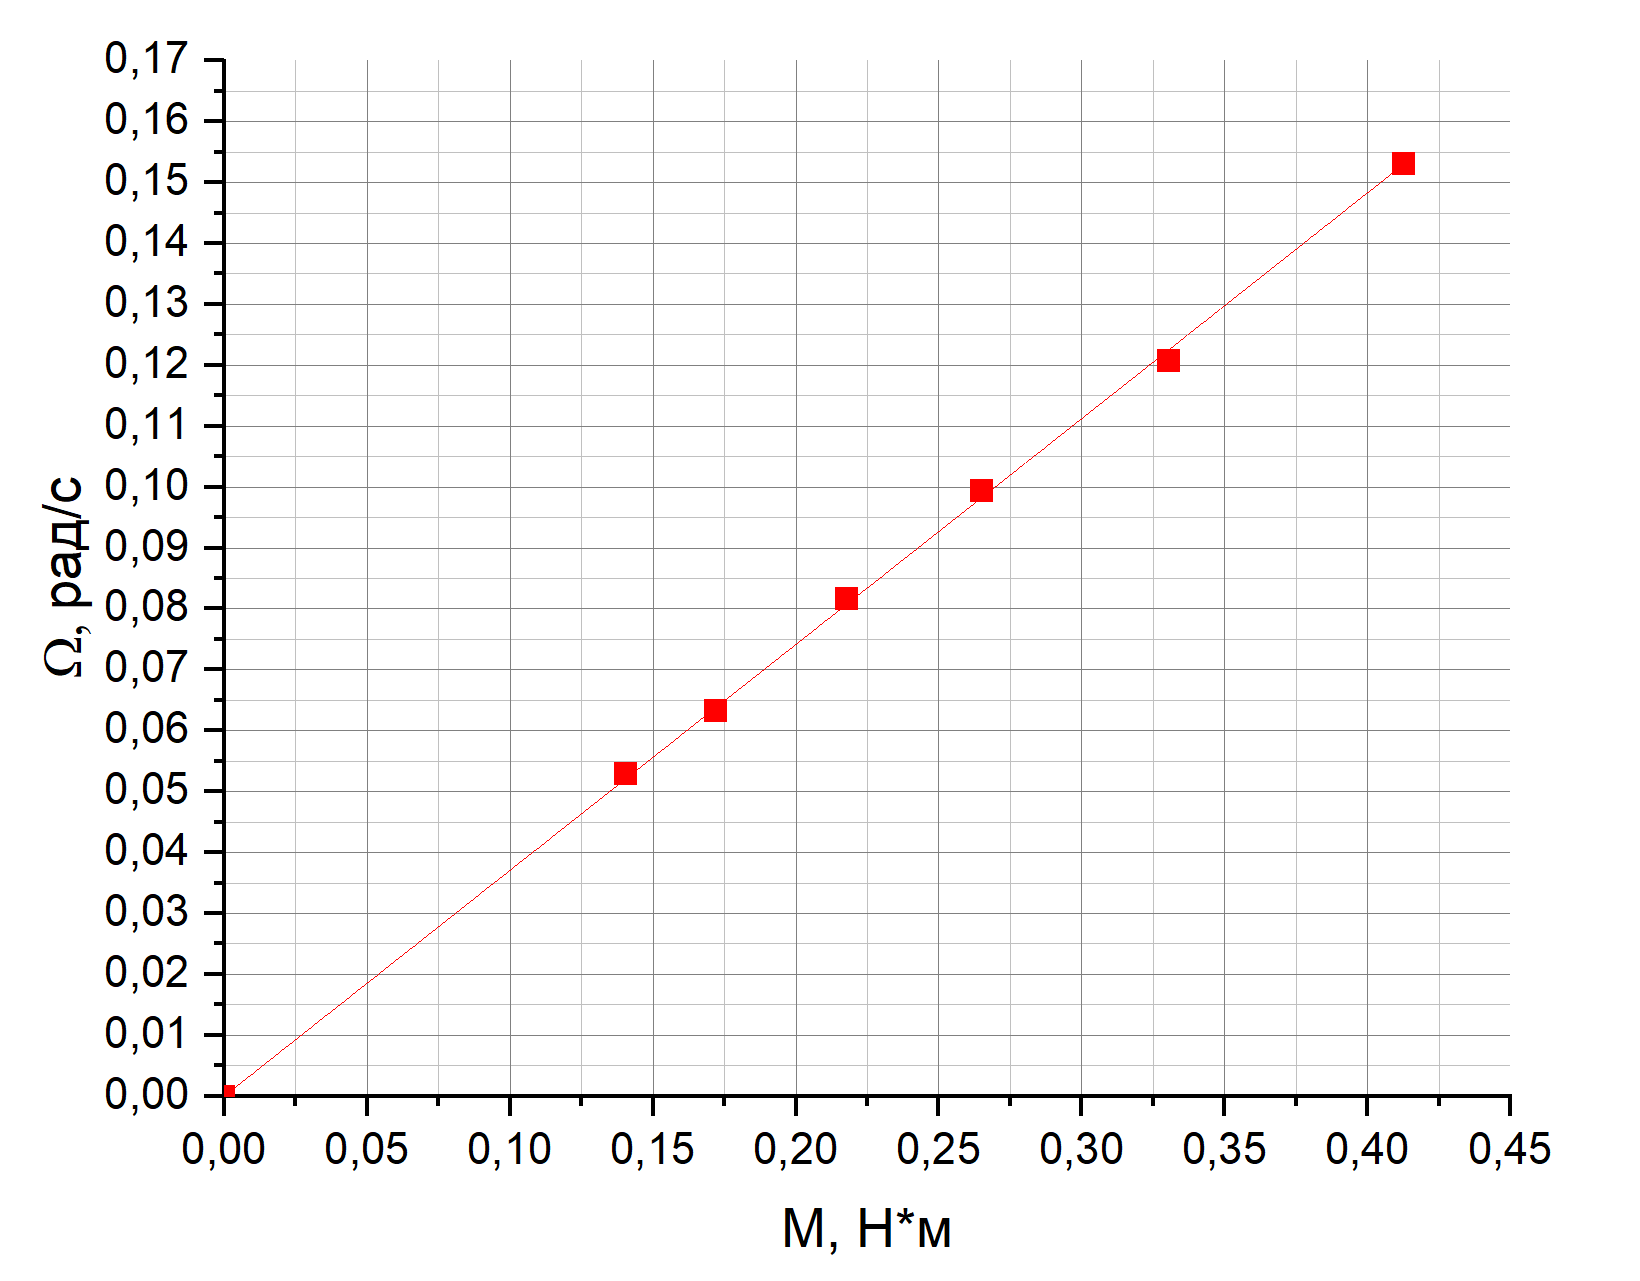
\includegraphics[scale=0.4]{4}
\caption{График зависимости угловой скорости регулярной прецессии гироскопа $\Omega$ от момента силы тяжести $M$, который создает грузик. }
\end{figure}
\newpage
Измерим диаметр цилиндра. Результаты занесем в Таблицу 3.
\begin{table}[h]
\centering
\begin{tabular}{|c|c|c|c|c|c|c|c|c|c|c|}
\hline
$\text{№}$    & 1    & 2    & 3    & 4    & 5    & 6  & 7    & 8    & 9    & 10 \\ \hline
d, мм & 78,2 & 78,1 & 78,1 & 78,3 & 78,2 & 78 & 78,1 & 78,1 & 78,2 & 78 \\ \hline
\end{tabular}
\caption{Измерение диаметраа цилиндра $d$}
\end{table}

Усредняя результаты получим, что
\[d = (78,13\pm0,13)\text{мм}\]
Посчитаем момент инерции по формуле:
\[I = \frac{m_\text{ц}d^2}{4}\]
\[I = (1,234\pm0,006)\cdot 10^{-3}\text{кг}\cdot \text{м}^2\]
Для нахождения момента инерции ротора измеряем период крутильных колебаний цилиндра и ротора $T$. Результаты заносим в таблицу 4. $N$ -- число колебаний. 
\begin{table}[h]
\centering
\begin{tabular}{|c|c|c|c|c|}
\hline
\multicolumn{5}{|c|}{Цилиндр}     \\ \hline
$N$ & 15    & 15    & 15    & 15    \\ \hline
$t, \text{с}$ & 64,81 & 64,63 & 64,75 & 64,66 \\ \hline
$T, \text{с}$ & 4,32  & 4,31  & 4,32  & 4,31  \\ \hline
\multicolumn{5}{|c|}{Ротор}       \\ \hline
$N$ & 20    & 20    & 20    & 20    \\ \hline
$t, \text{с}$ & 64,81 & 64,63 & 64,75 & 64,66 \\ \hline
$T, \text{с}$ & 3,24  & 3,23  & 3,24  & 3,23  \\ \hline
\end{tabular}
\caption{Период крутильных колебаний цилиндра и ротора}
\end{table}
Усредняя получим, что период крутильных колебаний цилиндра равен:
\[T_\text{ц} = (4,3\pm0,1)\text{c}\]
Период крутильных колебаний ротора:
\[T_0 = (3,24\pm0,1)\text{с}\]
Момент инерции вычисляем по формуле (10):
\[I_0 = I_\text{ц}\frac{T_0^2}{T_{\text{ц}}^2}\]
\[I = (0,69\pm0,05)\cdot 10^{-3}\text{кг}\cdot \text{м}^2\]

Расчитаем частоту вращения ротора гироскопа $\omega_0$ по формуле:
\[\omega_0 = \frac{M}{\Omega I_0}\]
\[\omega_0 = (604,2\pm47,6)\text{Гц}\]
Значение частоты, полученное на осциллографе:
\[\omega_0^0 = (487\pm28)\text{Гц}\]
Определим момент сил трения для грузика массой $m = 341\text{г}$ по скорости опускания рычага $\text{C}$ во время прецессии.
\[M_\text{тр} = I_0\omega_0\Omega_\text{тр}\]
\[M_\text{тр} = (0,085\pm0,009)\cdot 10^{-3}\text{кг}\cdot \text{м}\]
\section{Обсуждение результатов и выводы}
В работе была эксперементальна подтверждена прямопропорциональная зависимость между угловой скоростью регулярной прецессии гироскопа $\Omega$ и моментом силы тяжести $M$ (Рис. 3), что подтверждает формулу (8).

По графику было получено значение частоты вращения гироскопа
\[\omega_0 = (604\pm47)\text{Гц}\]
Также было получение значение частоты вращения гироскопа с помощью осциллографа:
\[\omega_0^0 = (487\pm28)\text{Гц}\]
Значения отличаются, что свидетельствует о неточности измерений.

Отношение момента слиы трения к моменту силы тяжести равно:
\[\frac{M_{mg}}{M_\text{тр}} \approx 5000\]
Это говорит о совсем незначительном влиянии силы трения на прецессию гироскопа.
\end{document}